\documentclass{article}

% if you need to pass options to natbib, use, e.g.:
%     \PassOptionsToPackage{numbers, compress}{natbib}
% before loading neurips_2018

% ready for submission
% \usepackage{neurips_2018}

% to compile a preprint version, e.g., for submission to arXiv, add add the
% [preprint] option:
%     \usepackage[preprint]{neurips_2018}

% to compile a camera-ready version, add the [final] option, e.g.:
     \usepackage[final]{neurips_2018}

% to avoid loading the natbib package, add option nonatbib:
%     \usepackage[nonatbib]{neurips_2018}

\usepackage[utf8]{inputenc} % allow utf-8 input
\usepackage[T1]{fontenc}    % use 8-bit T1 fonts
\usepackage{hyperref}       % hyperlinks
\usepackage{url}            % simple URL typesetting
\usepackage{booktabs}       % professional-quality tables
\usepackage{amsfonts}       % blackboard math symbols
\usepackage{nicefrac}       % compact symbols for 1/2, etc.
\usepackage{microtype}      % microtypography
\usepackage{graphicx}
\usepackage{float} 
\usepackage{subfigure}

\title{628 Final Project Report\\
Event Recommendation System}

% The \author macro works with any number of authors. There are two commands
% used to separate the names and addresses of multiple authors: \And and \AND.
%
% Using \And between authors leaves it to LaTeX to determine where to break the
% lines. Using \AND forces a line break at that point. So, if LaTeX puts 3 of 4
% authors names on the first line, and the last on the second line, try using
% \AND instead of \And before the third author name.

\author{%
  Xinghan Qin
  % examples of more authors
  % \And
  % Coauthor \\
  % Affiliation \\
  % Address \\
  % \texttt{email} \\
  % \AND
  % Coauthor \\
  % Affiliation \\
  % Address \\
  % \texttt{email} \\
  % \And
  % Coauthor \\
  % Affiliation \\
  % Address \\
  % \texttt{email} \\
  % \And
  % Coauthor \\
  % Affiliation \\
  % Address \\
  % \texttt{email} \\
}

\begin{document}
% \nipsfinalcopy is no longer used

\maketitle

\begin{abstract}
This report will discuss the whole processing of why and how to build Event Recommendation System, system performance analyse and future improvement.
\end{abstract}

\section{Introduction}

As life speed becomes faster and faster, people sometimes can feel lonely and bored but don’t know what to do. One of the reasons for this situation is because our world is too colourful. When people have too many interests, then sometimes it will become very hard for us to decide exactly what to do. And at the end, we will decide to do nothing.\\

Hence, because of this problem, I decided to create an events recommendation system to help people choose some events, that this person may interest to, based on the person information, friends list, and event attendance record. The data set was found on open source website, Kaggle. Following is the link:

\begin{center}
  \url{https://www.kaggle.com/c/event-recommendation-engine-challenge/data}
\end{center}

\section{Aims and Objectives}

\subsection{Aims}

Based on given events information, user information, training data and test data, to train a network to predict if the user will interest or uninterest to the event.

\subsection{Objectives}

•	Analyse the given data sets and select the features\\
•	Read and process data into wanted format\\
•	Create the model based on requirement\\
•	Train and evaluate the model by train data and validate data\\
•	Predict the result for test data

\section{Data Analyse}

\subsection{Data sets}

•	train.csv: (15398 * 6)\\
	user, event, invited, timestamp, interested, not\verb+_+interested\\
•	test.csv: (10237 * 4)\\
	user, event, invited, timestamp\\
•	users.csv: (38209 * 7)\\
	user\verb+_+id, locale, birthyear, gender, joinedAt, location, timezone\\
•	event\verb+_+attendees.csv: (24144 * 5)\\
	event, yes, maybe, invited, no\\
•	events.csv: (3137972 * 110)\\
	event\verb+_+id, user\verb+_+id, start time, city, state, zip, country, lat, lng, count\verb+_+1, count\verb+_+2, ..., count\verb+_+100, count\verb+_+other\\
•	user\verb+_+friends.csv: (38202 * 2)\\
	user\verb+_+id, friends
	
\subsection{Features}

•	user\verb+_+id: the id of the user\\
•	event\verb+_+id: the id of the event\\
•	interested: does user interest in the event\\
•	not\verb+_+interested: does user uninterested the event\\
•	invited: have user been invited, 1 for yes, 0 for no\\
•	friend\verb+_+attend\verb+_+yes: the number of friends attend the event\\
•	friend\verb+_+attend\verb+_+maybe: the number of friends maybe attend the event\\
•	friend\verb+_+attend\verb+_+invited: the number of friends invited to the event\\
•	friend\verb+_+attend\verb+_+no: the number of friends not attend the event\\
•	attend\verb+_+same\verb+_+genderrate\verb+_+yes: the rate of same gender attends the event\\
•	attend\verb+_+same\verb+_+gender\verb+_+rate\verb+_+maybe: the rate of same gender maybe attends the event\\
•	attend\verb+_+same\verb+_+gender\verb+_+rate\verb+_+invite: the rate of same gender invites by the event\\
•	attend\verb+_+same\verb+_+gender\verb+_+rate\verb+_+no: the rate of same gender not attend the event\\
•	host\verb+_+is\verb+_+friend: is host is friend of user, 1 for yes, 0 for no\\
•	c\verb+_+1 to c\verb+_+100: the information about the event\\
•	interest\verb+_+c1 to interest\verb+_+c\verb+_+100: the mean value of user attended events’ information\\

More features will be added in the future. The information about time, location and time zone has not been applied. 


\section{Data Processing}

\subsection{Read data}

To read and use given data sets efficiently, 7 dictionaries were designed:\\
("1": yes, "2": maybe, "3": invited, "4": no)

•	train\verb+_+dict = \verb+{+user\verb+_+id : \verb+{+event\verb+_+id : [invited, interested, not\verb+_+interested]\verb+}+\verb+}+\\
•	test\verb+_+dict = \verb+{+user\verb+_+id : \verb+{+event\verb+_+id : invited\verb+}+\verb+}+\\
•	friends\verb+_+dict = \verb+{+user\verb+_+id : []\verb+}+\\
•	users\verb+_+dict = \verb+{+user\verb+_+id : [birthday, gender]\verb+}+\\
•	events\verb+_+dict = \verb+{+event\verb+_+id : [host\verb+_+user\verb+_+id, [c\verb+_+list]]\verb+}+\\
•	user\verb+_+interests\verb+_+dict = \verb+{+user\verb+_+id : \verb+{+"1" : [], "2" : [], "3" : [], "4" : []\verb+}+\verb+}+\\
•	event\verb+_+attendees\verb+_+dict = \verb+{+event\verb+_+id : \verb+{+"1" : [], "2" : [], "3" : [], "4" : []\verb+}+\verb+}+\\

During reading the data, Duplicated data in user was found, and shows in Figure 1 and Figure 2. Because it was just duplicated and had no multiple data for same combo of user and event, the data will be ignored if it just duplicated. Hence, after processing, the train\verb+_+data and test\verb+_+data would be 15398 – 178 and 10237 – 131 and result shows in Figure 3.

\begin{figure}[h]
  \centering
  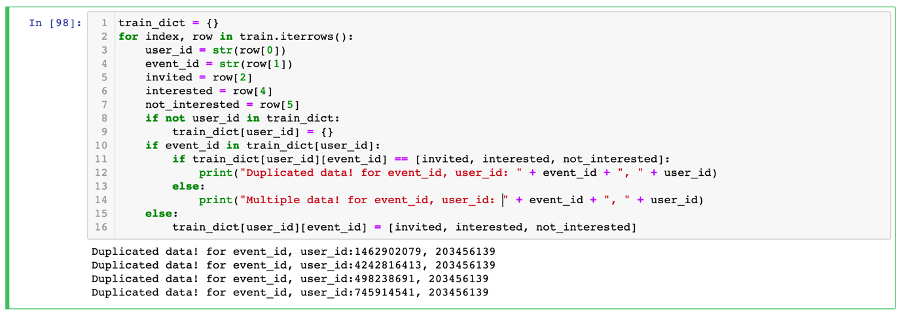
\includegraphics[width=1.0\textwidth]{img/Picture 2}
  \caption{Duplicated data}
\end{figure}

\begin{figure}[h]
  \centering
  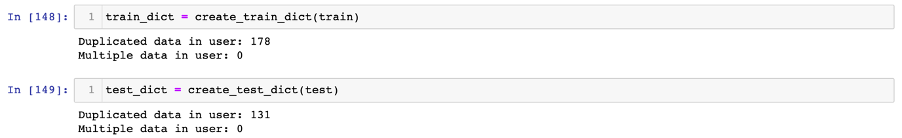
\includegraphics[width=1.0\textwidth]{img/Picture 1}
  \caption{Amount of d duplicated data}
\end{figure}

\begin{figure}[h]
  \centering
  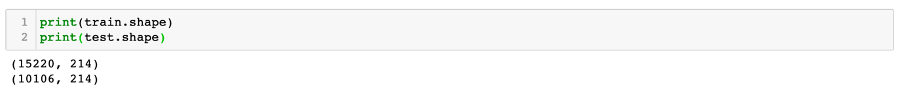
\includegraphics[width=1.0\textwidth]{img/Picture 0}
  \caption{Size of training and testing data}
\end{figure}

\subsection{Data processing}

As all data has been read into the dictionary, train\verb+_+data and test\verb+_+data should be create based on the feature design.

•	user\verb+_+id: \\
	train\verb+_+dict.keys()\\
•	event\verb+_+id: \\
	train\verb+_+dict[user\verb+_+id].keys()\\
•	interested: \\
	train\verb+_+dict[user\verb+_+id][event\verb+_+id][1], for test\verb+_+data is -1\\
•	not\verb+_+interested: \\
	train\verb+_+dict[user\verb+_+id][event\verb+_+id][2], for test\verb+_+data is -1\\
•	invited: \\
	train\verb+_+dict[user\verb+_+id][event\verb+_+id][0]\\
•	friend\verb+_+attend\verb+_+yes, friend\verb+_+attend\verb+_+maybe, friend\verb+_+attend\verb+_+invited, friend\verb+_+attend\verb+_+no: \\
	attend\verb+_+list = event\verb+_+attendees\verb+_+dict[event\verb+_+id]\\
	friends\verb+_+list = friends\verb+_+dict[user\verb+_+id]\\
	compare attend\verb+_+list with friends\verb+_+list\\
•	attend\verb+_+same\verb+_+gender\verb+_+rate\verb+_+yes, attend\verb+_+same\verb+_+gender\verb+_+rate\verb+_+maybe, attend\verb+_+same\verb+_+gender\verb+_+rate\verb+_+invite, attend\verb+_+same\verb+_+gender\verb+_+rate\verb+_+no: \\
	attend\verb+_+list = event\verb+_+attendees\verb+_+dict[event\verb+_+id]\\
	gender = users\verb+_+dict[guest\verb+_+id in attend\verb+_+list]\\
•	host\verb+_+is\verb+_+friend: \\
	friends\verb+_+list = friends\verb+_+dict[user\verb+_+id]\\
	host\verb+_+id = events\verb+_+dict[event\verb+_+id][0]\\
•	c\verb+_+1 to c\verb+_+100:\\
	events\verb+_+dict[event\verb+_+id][1 : 100]\\
•	interest\verb+_+c1 to interest\verb+_+c\verb+_+100:\\
	interests\verb+_+list = user\verb+_+interests\verb+_+dict[user\verb+_+id]\\
	mean of all events\verb+_+dict[event\verb+_+id in interests\verb+_+list][1 : 100]\\
	
During the data processing, some problems about the data set were found. The main problem was lack of data. For example, lots of user\verb+_+id in event\verb+_+attendees cannot be found in users file. Hence, while processing the same gender, there were lots of unknown data. This situation also happened for user\verb+_+interests\verb+_+dict. Some user didn’t attend any events before, hence, there was not record for the interest. Because lack of data happens in real world as well, unknown data was ignored or tread as 0 this time depends on the situation.

\subsection{Result}

train\verb+_+data.csv will be showed in Figure 4. test\verb+_+data.csv will be showed in Figure 5.

\begin{figure}[h]
  \centering
  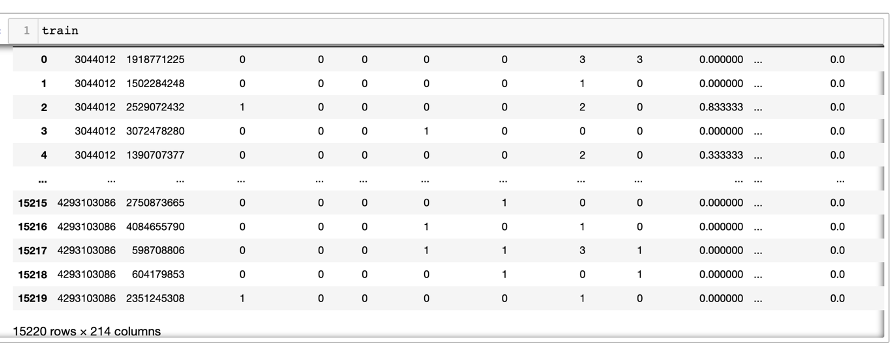
\includegraphics[width=1.0\textwidth]{img/Picture 3}
  \caption{Train data}
\end{figure}
\begin{figure}[h]
  \centering
  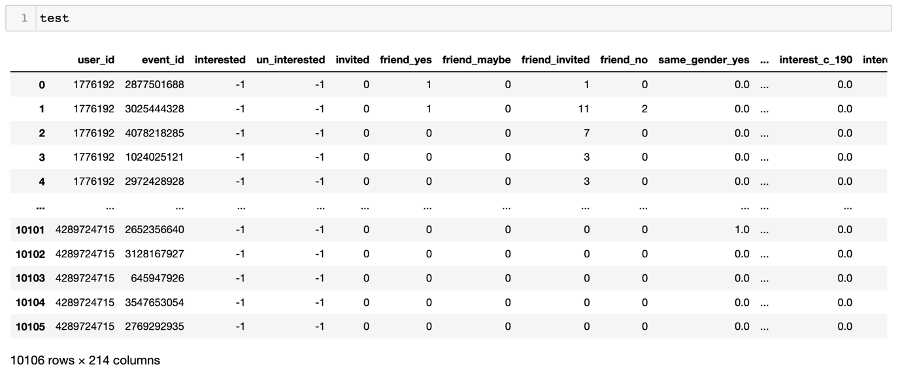
\includegraphics[width=1.0\textwidth]{img/Picture 4}
  \caption{Test data}
\end{figure}

\section{Model Training}

\subsection{Data prepare}

Total training data set has 15220 elements, 14000 elements were set as training data and the rest data were set as validation data. Total test data set has 10106 elements, Figure 6.

\begin{figure}[h]
  \centering
  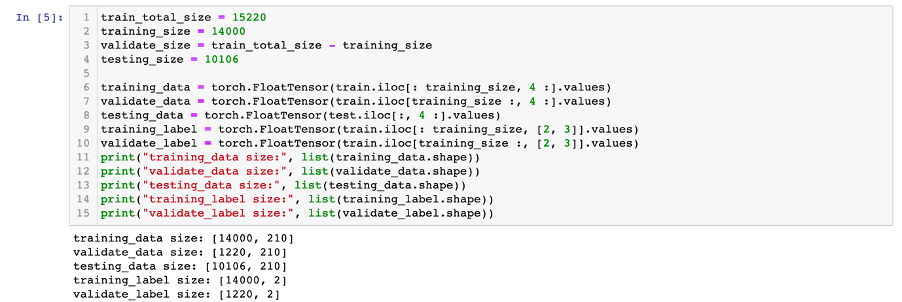
\includegraphics[width=1.0\textwidth]{img/Picture 5}
  \caption{Size of all data sets}
\end{figure}

\subsection{Model setting}

First hidden layer: input size 210, output size 514, linear and ReLU\\
Second hidden layer: input size 514, output size 128, linear and ReLU\\
Output layer: input size 128, output size 2, linear

\begin{figure}[h]
  \centering
  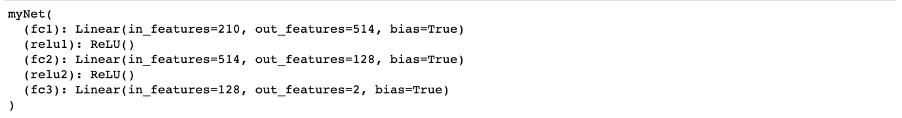
\includegraphics[width=1.0\textwidth]{img/Picture 6}
  \caption{Model}
\end{figure}

Optimizer and loss function in Figure 8

\begin{figure}[h]
  \centering
  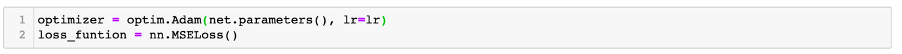
\includegraphics[width=1.0\textwidth]{img/Picture 7}
  \caption{Optimizer and loss function }
\end{figure}

Depends on the batch\verb+_+size to create train\verb+_+loader in Figure 9

\begin{figure}[h]
  \centering
  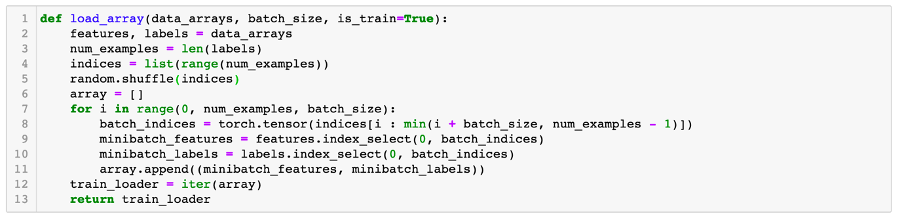
\includegraphics[width=1.0\textwidth]{img/Picture 8}
  \caption{Train loader }
\end{figure}

Depends on Epochs to train the model, and print the loss for this epoch in Figure 10

\begin{figure}[h]
  \centering
  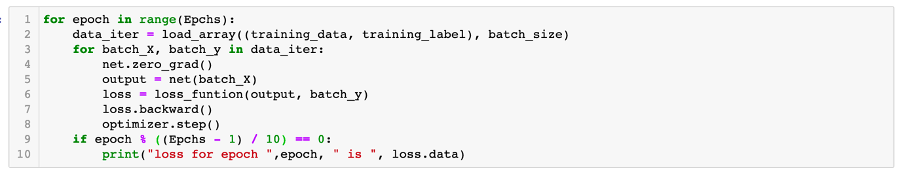
\includegraphics[width=1.0\textwidth]{img/Picture 9}
  \caption{Training circle}
\end{figure}

\subsection{Parameters setting}

To improve the model, batch\verb+_+size, learning rate(lr) and Epchs were adjusted based on the final epoch loss and AUC of results.

For batch\verb+_+size = 140, lr = 0.01, Epchs = 101:\\
As Figure 11 shows, the final epoch loss was 0.0546. And during the training, the loss didn’t get improved gradually. Hence, lr was decided to be decreased.

For batch\verb+_+size = 140, lr = 0.001, Epchs = 101:\\
In Figure 12, as lr was decreased, the loss has been decreased. However, because in the training data, there were lots of 0 (the reason will be discus in the next part). batch\verb+_+size was increased to avoid all data in batch were 0.

For batch\verb+_+size = 1400, lr = 0.001, Epchs = 101:\\
As Figure 13 shows, the loss increased. However, different than before, the loss kept tend of decrease. The previous results tended to be stable or jump back. To determine when would the results tended to be stable or jump back, Epchs was increased.

For batch\verb+_+size = 1400, lr = 0.001, Epchs = 1001:\\
As Figure 14 shows, the loss was decreased. However, although the AUC of training\verb+_+data\verb+_+pred became 0.994, which means the model is very close to the training data, the AUC of validation data decreased to 0.538. This caused by overfitting. Because the model has been trained too many times, the model almost kept the shape of training data. Hence, Epchs needed to be decreased. As the part be highlighted shows, during 700th epoch, the loss has jumped back. Hence, Epchs was set somewhere around 600.

For batch\verb+_+size = 1400, lr = 0.001, Epchs = 651:\\
As Figure 15 shows, the loss was 0.0184, and AUC of validation data was 0.581. Hence, the model has been improved, and this would be the final version of the model.

\section{Result Analyse}

As the final result shows, the final AUC of validation data was 0.581 and loss was 0.2, which was one of the best results and parameter setting for this model. However, this result did not match the expectation. Following are the reasons may cause this situation:

•	Lack of data:\\
	While processing the training\verb+_+data and testing\verb+_+data based the features been designed, there were lots of unknow data. For lots of user\verb+_+id in friends\verb+_+list, no information can be found according to user\verb+_+id in users.csv. This means lots of the numbers of friend’s attendance for the user were 0. Also, for user\verb+_+id in attended.csv had same issue. For the user in training data, lots of them did not have any record of the event attendance. Hence, the result for interest\verb+_+c\verb+_+1 to interest\verb+_+c\verb+_+100 could all be 0. The lack of data caused training data included many 0.
	
•	Unused data:\\
	In the original data set, there were some data this model didn’t apply. Those data were mainly location, timestamp, birthday and time zone. For those data, some needed higher skill to processing. Like location, the given data in same column has different format. Some were city and status, and some others were status and country. Hence, need other tool to determine the information. And for data like timestamp, with limited knowledge, those data cannot be transfer into useful data. Put timestamp in integer, like 20200314, into training data was not meaningful. Hence, some of unused data may be important features for model. However, based on limited skill and knowledge, those data have not been applied.
	
•	Model:\\
	The model can be more complicated by applying different type of method.
	
•	Parameters:\\
	More testing should be done to improve the parameters.\\

\section{Future Improvement}

As been discussed in Result analyse, following are the future improvement:

•	Search for more data set to complete the training data (the data was found on Kaggle, hence this is not doable)\\
•	Apply more data in the original data set, learn more skill and theory to represent these data\\
•	Complicate the model by using more methods\\
•	Do more testing to improve the parameters\\

\section{Conclusion}

For this event recommendation system model, it has 214 features, the loss of training data was 0.0184, the AUC of training data was 0.993, the loss for validation data was 0.2 and AUC of validation data was 0.831. Although the trained model did not have high performers, the improve directions have been found out. With more self-learning, it will have more useful features, more data, more complicated model and better parameters. 

\begin{figure}[h]
  \centering
  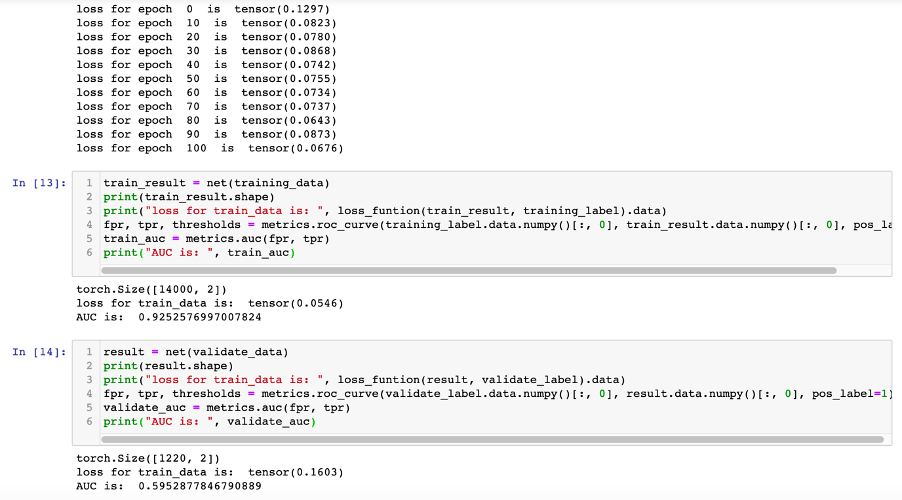
\includegraphics[width=1.0\textwidth]{img/Picture 10}
  \caption{140, 0.01, 101}
\end{figure}

\begin{figure}[h]
  \centering
  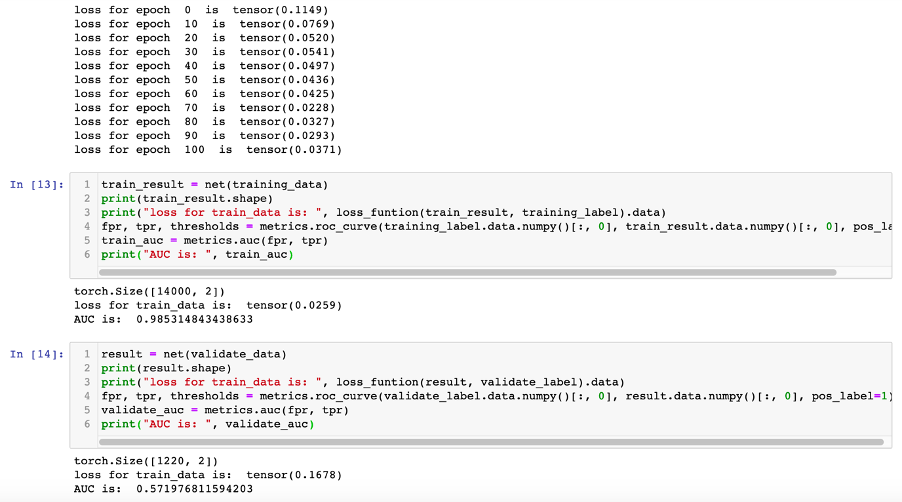
\includegraphics[width=1.0\textwidth]{img/Picture 11}
  \caption{140, 0.001, 101}
\end{figure}

\begin{figure}[h]
  \centering
  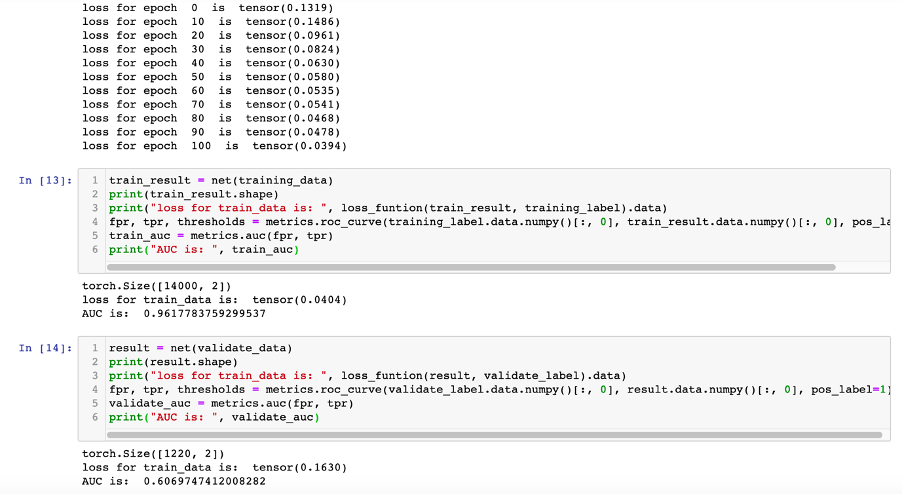
\includegraphics[width=1.0\textwidth]{img/Picture 12}
  \caption{1400, 0.001, 101}
\end{figure}

\begin{figure}[h]
  \centering
  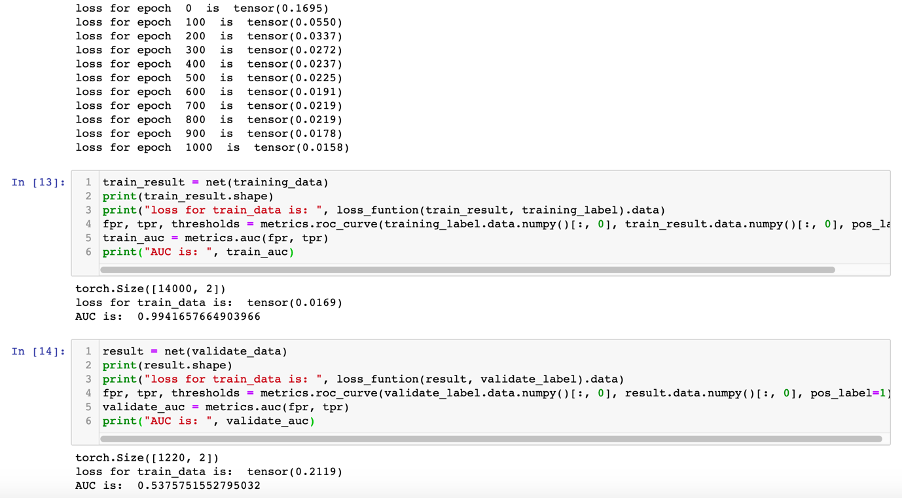
\includegraphics[width=1.0\textwidth]{img/Picture 13}
  \caption{1400, 0.001, 1001}
\end{figure}

\begin{figure}[h]
  \centering
  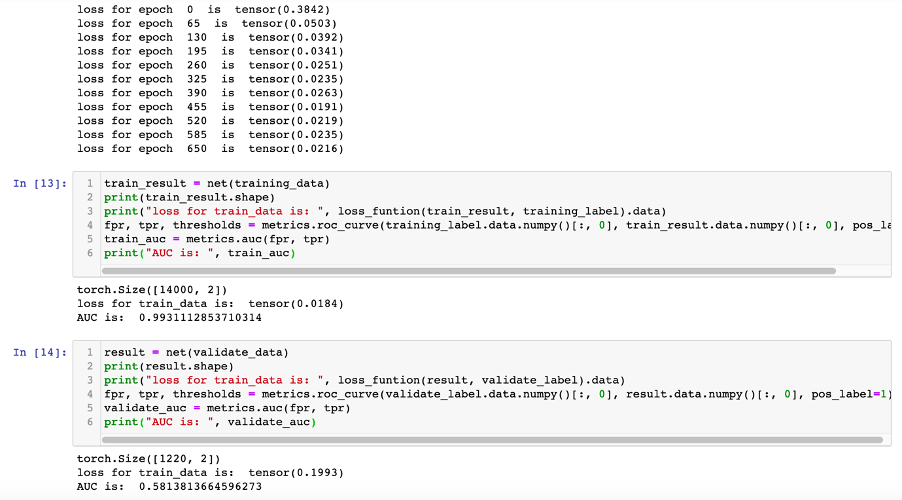
\includegraphics[width=1.0\textwidth]{img/Picture 14}
  \caption{1400, 0.001, 651}
\end{figure}

\end{document}
